\section{Algoritmi non supervisionati}
A differenza degli algoritmi supervisionati, in quelli non supervisionanti per ciascun esempio non è nota l'uscita, cioè la sua classe di appartenenza, e dunque non è possibile effettuare una fase di \emph{training}. Lo scopo di questi algoritmi può essere quello di raggruppare esempi simili (\emph{clustering}) oppure ridurre la dimensionalità dei vettori delle \emph{feature} (\emph{dimensionality reduction}).

\subsection{Clustering}
Lo scopo del \emph{clustering} è raggruppare in maniera ``naturale'' le istanze fornite. Si punta quindi a creare dei \emph{cluster} a cui appartengano degli elementi che condividono alcune proprietà e che, dunque, sono simili tra loro. Le proprietà che caratterizzano un \emph{cluster} sono due:
\begin{itemize}
\item alta similarità \emph{intra-cluster}, cioè tra istanze appartenenti allo stesso \emph{cluster} (che pertanto si dirà ``omogeneo'');
\item bassa similarità \emph{inter-cluster}, cioè tra istanze appartenenti a \emph{cluster} distinti.
\end{itemize}

Gli algoritmi di \emph{clustering} si distinguono in \emph{hard} e \emph{soft clustering}:
\begin{itemize}
\item si parla di \emph{hard clustering} quando l'algoritmo determina la classe di appartenenza di un'istanza, senza dare alcuna informazione su quanto è probabile che quella sia la reale classe di appartenenza;
\item si parla di \emph{soft clustering} quando l'algoritmo indica, per ciascuna istanza, qual è la probabilità che appartenga a ciascun \emph{cluster}.
\end{itemize}

\subsubsection{K-means}\label{sec:k-means}
Si tratta di un semplice algoritmo di \emph{hard clustering} che si articola nelle seguenti fasi:
\begin{enumerate}
\item fissa il numero di \emph{cluster} $K$ in maniera casuale o basandoti su un euristica nota;
\item scegli casualmente $K$  punti tra le istanze note ed assumi che siano i centroidi dei $K$  \emph{cluster};
\item\label{step:assegna_cluster} assegna ogni rimanente punto al \emph{cluster} il cui centroide è più vicino (per valutare la distanza si può usare una distanza Euclidea, di Manhattan o altro ancora);
\item in base ai campioni aggiunti in ciascun \emph{cluster} ricalcola la posizione dei centroidi\footnote{Ciascuna coordinata del centroide di un \emph{cluster} è calcolata come la media del valore che tale coordinata assume per tutti i punti del \emph{cluster}.};
\item torna al~\autoref{step:assegna_cluster} fino al raggiungimento della condizione di convergenza.
\end{enumerate}
La condizione di convergenza può essere un numero massimo di iterazioni oppure il momento in cui ciascun centroide dista dal suo valore precedente di una quantità minore ad una soglia desiderata. Al termine dell'algoritmo avremo minimizzato la distanza quadratica media delle istanze dai rispettivi centroidi, detta anche \emph{dispersione}:
\begin{equation*}
J(c^{(1)}, \dots,c^{(m)},\mu_1, \dots,\mu_K) = \frac{1}{m} \sum_{i=1}^m || x^{(i)} - \mu_{c^{(i)}} ||^2
\end{equation*}
in cui:
\begin{itemize}
\item $m$ è il numero complessivo di istanze;
\item $ x^{(i)}$ è la \emph{i-esima} istanza;
\item $c^{(i)}$ è il \emph{cluster} a cui appartiene il punto $x^{(i)}$;
\item $\mu_{c^{(i)}}$ sono le coordinate del centroide del \emph{cluster} a cui appartiene $ x^{(i)}$;
\item $|| x^{(i)} - \mu_{c^{(i)}} ||^2$ è la distanza quadratica tra ciascuna istanza ed il suo centroide.
\end{itemize}
Si dimostra matematicamente che il primo primo passo dell'algoritmo, quello in cui assegnamo ciascun punto ad un cluster, minimizza la funzione costo variando $c^{(i)}$, mentre il secondo passo, in cui aggiorniamo i centroidi, la minimizza variando i $\mu_k$.


Un vantaggio di questo algoritmo è costituito dalla sua semplicità, ma presenta alcuni svantaggi, tra cui:
\begin{itemize}
\item\emph{ Non è adatto per dati di tipo categoriale}. Per funzionare, infatti, è necessario poter stabilire una distanza tra due generiche istanze. Affinché ciò sia possibile i vettori delle \emph{feature} devono essere numerici, o quantomeno dobbiamo essere in grado di applicare una metrica di distanza tra coppie di istanze.
\item\emph{Necessita di specificare $K$ in anticipo}. In questa categoria di problemi non abbiamo informazioni a priori su quali e quante classi cercare, quindi diventa difficile indovinare il $K$ esatto fin da subito. Una possibilità è avviare più volte l'algoritmo con $K$ diversi e confrontare i risultati. Vedremo a breve come si può realizzare ciò.
\item\emph{Può restare bloccato in minimi locali}. Ad esempio può accadere quanto mostrato in \autoref{fig:k-means-minimo-locale}, nella quale in quello che dovrebbe essere un unico \emph{cluster} è possibile individuare sottogruppi di istanze molto simili che agli occhi dell'algoritmo appaiono come \emph{cluster} distinti. La \emph{clusterizzazione} che ne consegue è palesemente errata.
\item\emph{Molto sensibile a rumore ed outlier}. Se, casualmente, un \emph{outlier} fosse scelto come centroide iniziale, questo potrebbe influire negativamente sul resto dell'algoritmo. Per ovviare a ciò si può rilanciare \emph{k-means} più volte e vedere a che risultati porta.
\item\emph{Non adatto a cluster con forme non convesse}.
\end{itemize}


\begin{figure}[tbp]
\centering
  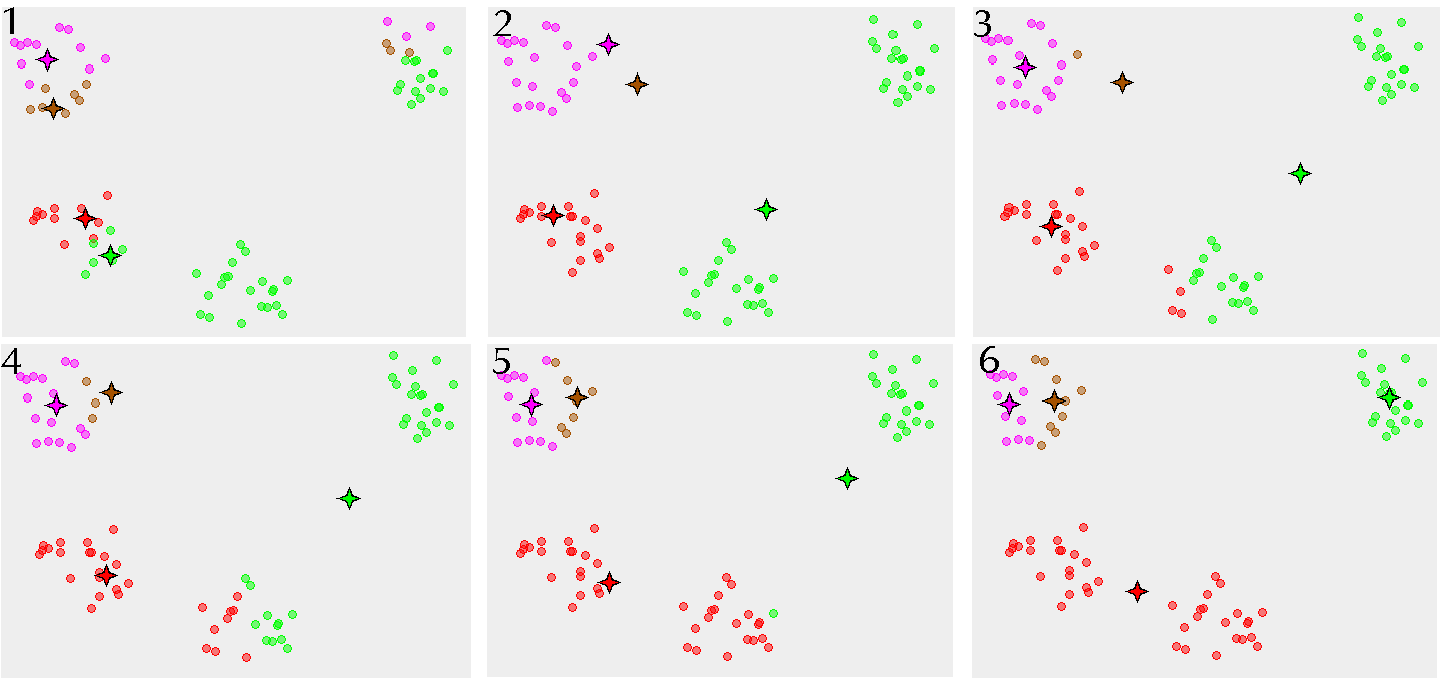
\includegraphics[width = \textwidth]{images/k-means-minimo-locale}
  \caption{K-Means converge in un minimo locale}
  \label{fig:k-means-minimo-locale}
\end{figure}

Abbiamo visto che uno dei punti delicati del \emph{k-means} è la scelta di $K$. Per capire quale sia il valore ottimo è possibile variare $K$ e \emph{plottare} il valore della funzione costo in funzione di essa\footnote{A volte si usa la  \emph{Within Groups Sum of Squares} che è identica a $J(K)$ ma non normalizzata rispetto al numero di punti.}. Un valore troppo alto di $J(K)$ ci indica, ad esempio, che il \emph{clustering} non è significativo perché due o più \emph{cluster} potrebbero essere stati raggruppati attorno ad un unico centroide. Un valore troppo basso, però, è indice del fatto che abbiamo usato un numero troppo elevato di centroidi. Nel caso estremo avremo tanti centroidi quanti punti e questo porterà ad avere errore nullo. Tipicamente si può vedere che l'andamento di $J$ è decrescente (simile a quello in \autoref{fig:j(k)}) e si assume che il valore vero di $K$ coincida con il ginocchio di tale curva (cioè il punto in cui la pendenza comincia ad essere meno ripida, determinato tramite un'opportuna famiglia di algoritmi).

\begin{figure}[tbp]
\centering
  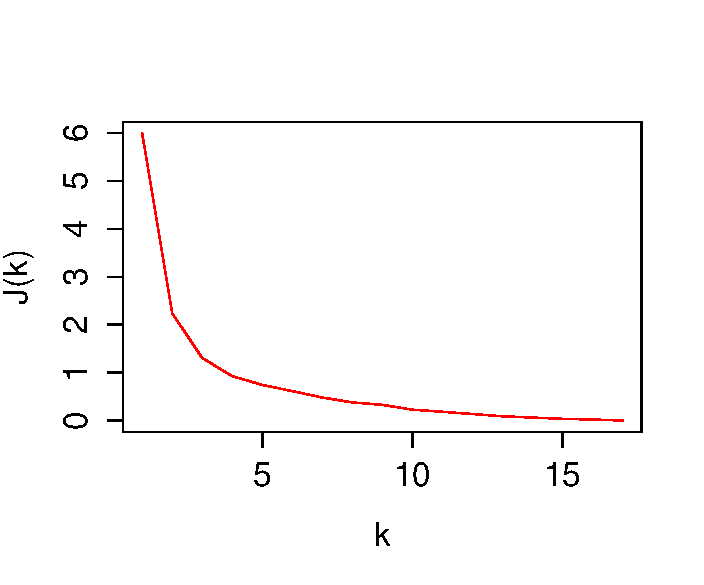
\includegraphics[width=0.7\textwidth]{images/jk}
  \caption{Andamento tipico della misura di distorsione dei cluster in funzione del numero di centroidi.}
  \label{fig:j(k)}
\end{figure}


\subsection{Principal Component Analysis}
\subsubsection{In sintesi}
Lo scopo di questa tecnica è passare da una rappresentazione delle istanze in $n$ variabili ad una rappresentazione in $p$ variabili \emph{latenti} (con $p<<n$). Nota bene che queste variabili sono \emph{latenti}, cioè non si tratta semplicemente di eliminare alcune \emph{feature} da quelle iniziali, ma di applicare un modello (lineare) alle \emph{feature} per \emph{proiettarle} in un nuovo dominio con dimensionalità inferiore. Questo nuovo dominio sarà caratterizzato da alcuni assi cartesiani, le coordinate di ciascun punto secondo il nuovo sistema di riferimento possono essere ottenute proiettando ciascun punto su ciascun asse. Le proiezioni dei punti su ciascun asse daranno luogo ad una distribuzione di valori e per ciascun asse è possibile calcolare la varianza di tale distribuzione. Poiché una varianza maggiore è indice del fatto che quella componente \emph{discrimina} maggiormente i punti, saremo interessati a prendere in considerazione solo le $p$ componenti a varianza maggiore (componenti principali). In questa maniera passiamo da una matrice degli ingressi di dimensione $m \times n$ ad una di dimensione $m \times p$. L'idea alla base delle tecniche di questo tipo è che le variabili osservabili siano in qualche maniera correlate e derivabili tutte da un insieme (più piccolo) di variabili latenti.

Capiamo meglio il concetto con un esempio. In~\autoref{fig:esempio_pca} sono mostrati alcuni punti, ciascuno dei quali è rappresentato da una coppia di valori $<x_1, x_2>$. La PCA ci consente di passare da una rappresentazione in $\mathcal{R}^2$ ad una rappresentazione in $\mathcal{R}$ (scegliendo $p=1$). Le componenti individuate dall'algoritmo (in seguito vedremo come) sono $u_1$ ed $u_2$. Proiettando i punti su $u_1$ ed $u_2$ ci rendiamo conto che la varianza delle proiezioni su $u_1$ è maggiore. Concludiamo che sarà questo asse la \emph{componente principale} ricercata e sarà sufficiente a descrivere il \emph{set} di istanze. In questo semplice esempio è facile capire che quanto fatto sia corretto, infatti tra $x_1$ ed $x_2$ sembra esserci una relazione lineare, e tra due variabili linearmente dipendenti è sufficiente conoscerne una per non perdere alcuna informazione (in questo caso la lineare dipendenza non è perfetta, quindi preserviamo gran parte dell'informazione, ma non tutta).

\begin{figure}[tbp]
\centering
  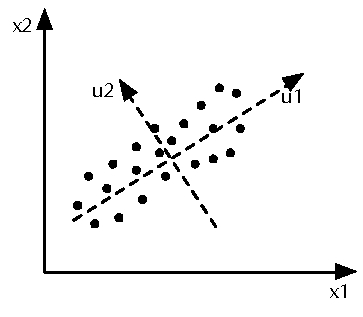
\includegraphics{images/esempio_pca}
  \caption{Esempio PCA}
  \label{fig:esempio_pca}
\end{figure}

\subsubsection{Passi necessari per la PCA}
Descriviamo quali passi sono necessari per portare a termine la PCA.

La prima operazione da fare è l'\emph{azzeramento del valor medio}, cioè a ciascuna \emph{feature}, di ciascuna istanza, sottraiamo il valor medio della stessa \emph{feature} calcolato su tutte le istanze. Passiamo quindi da
\begin{equation*}
x^{(i)}_1, x^{(i)}_2, \dots, x^{(i)}_n \qquad i = 1, \dots, m
\end{equation*}
a
\begin{equation*}
x^{(i)}_1 - \mu_1, x^{(i)}_2-\mu_2, \dots, x^{(i)}_n-\mu_n \qquad i = 1, \dots, m
\end{equation*}
con
\begin{equation*}
\mu_j = \frac{1}{m}\sum_{i=1}^m x^{(i)}_j.
\end{equation*}

Calcoliamo poi la matrice di covarianza ($\Sigma$) tra tutte le possibili coppie di \emph{feature}, il cui singolo elemento è così definito:
\begin{dmath*}
\Sigma_{ij} = \cov(x_i, x_j)
= E[(x_i-\mu_i)(x_j-\mu_j)]
= E[(x_i)( x_j)]
\end{dmath*}
Ricordiamo che la covarianza tiene conto di quanto due variabili aleatorie variano insieme, cioè di quanto sono simili nel loro comportamento.

Ora occorre conoscere autovalori ed autovettori della matrice delle covarianze. Per fare ciò applichiamo la \emph{Singular Value Decomposition} (SVD), anche nota come \emph{Decomposizione in Valori Singolari}, alla matrice $\Sigma$. Si tratta di una particolare fattorizzazione che, partendo da una matrice $A\in\mathbb{C}^{m\times n}$ ci consente di scrivere:
\begin{equation*}
A = U S V^*
\end{equation*}
dove:
\begin{itemize}
\item $U$ è una matrice unitaria sinistra di dimensioni $ m \times m$, cioè tale che moltiplicandola per la sua trasposta coniugata si ottiene la matrice identità ($U U^* = I$). Questa proprietà, nel caso di matrici reali, si traduce in $U^{-1} = U^T$;
\item $S$ è una matrice diagonale di dimensioni $m\times n$ (dove solo i primi $n$ elementi sono non nulli e costituiscono gli autovalori di A);
\item $V^*$ è la trasposta coniugata di una matrice unitaria di dimensioni $n\times n$.
\end{itemize}
Ricordiamo che la trasposta coniugata di una matrice si ottiene trasponendone gli elementi e sostituendo ciascuno di essi con il suo complesso coniugato (l'ordine delle due operazioni è irrilevante).

Gli elementi sulla diagonale principale di $S$ rappresentano gli autovalori di $A$, posti in ordine di valore decrescente man mano che ci si sposta verso il basso. Le colonne della matrice $U$  rappresentano gli autovettori sinistri di $A$ (cioè i vettori $\mathbf{u}$ t.c. $\mathbf{u}A=\mathbf{u}\lambda$ con $\lambda$ autovalore) e le colonne della matrice $V$ (e non $V^*$) rappresentano gli autovettori destri di $A$ (calcolati come $A\mathbf{v}=\lambda\mathbf{v} $). Nel caso di matrici simmetriche (come la matrice delle covarianze) questi autovalori coincidono, e quindi $U=V$. 

Ciò che si fa nel caso della PCA è applicare la SVD alla matrice delle covarianze:
\begin{equation*}
\Sigma = U S V^*
\end{equation*}
a questo punto di tutti gli autovalori che compaiono in $S$ ci interessa conservare solo i primi $p$, per questi autovalori consideriamo i corrispondenti autovettori. Ciascun autovettore sarà costituito da $n$ elementi, avremo quindi una matrice degli autovettori di dimensione $n \times p$.
Moltiplicare la matrice degli ingressi per l'autovettore \emph{i-esimo} significa calcolare il valore della coordinata \emph{i-esima} di ciascun ingresso rispetto al nuovo sistema di riferimento. Quindi moltiplicare la matrice degli ingressi ($m \times n$) per l'intera matrice degli autovettori ($n \times p$) equivale ad effettuare il cambio di coordinate richiesto per tutti gli ingressi. Il risultato sarà la nuova matrice dei campioni di dimensione ridotta ($m \times p$).

\begin{figure}
\centering
\begin{subfigure}[b]{0.5\textwidth}
\centering
  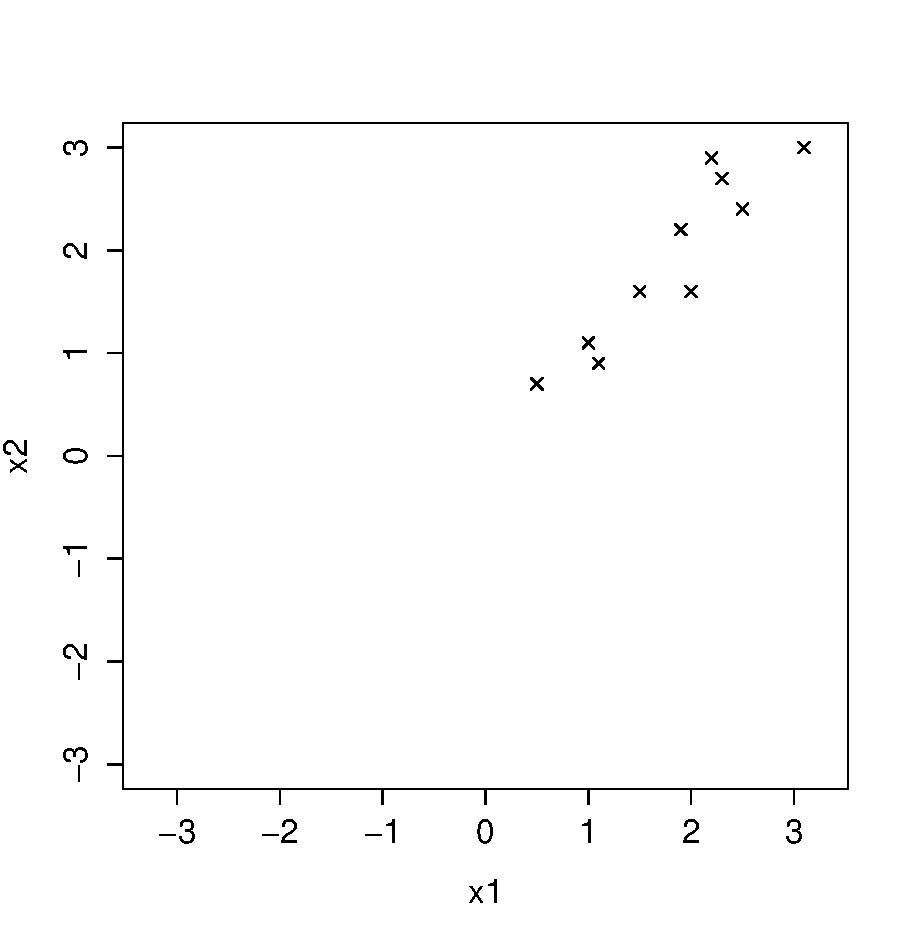
\includegraphics[width=\columnwidth]{images/points}
  \caption{Punti iniziali}
  \label{fig:punti_iniziali}
\end{subfigure}%
\begin{subfigure}[b]{0.5\textwidth}
    \centering
  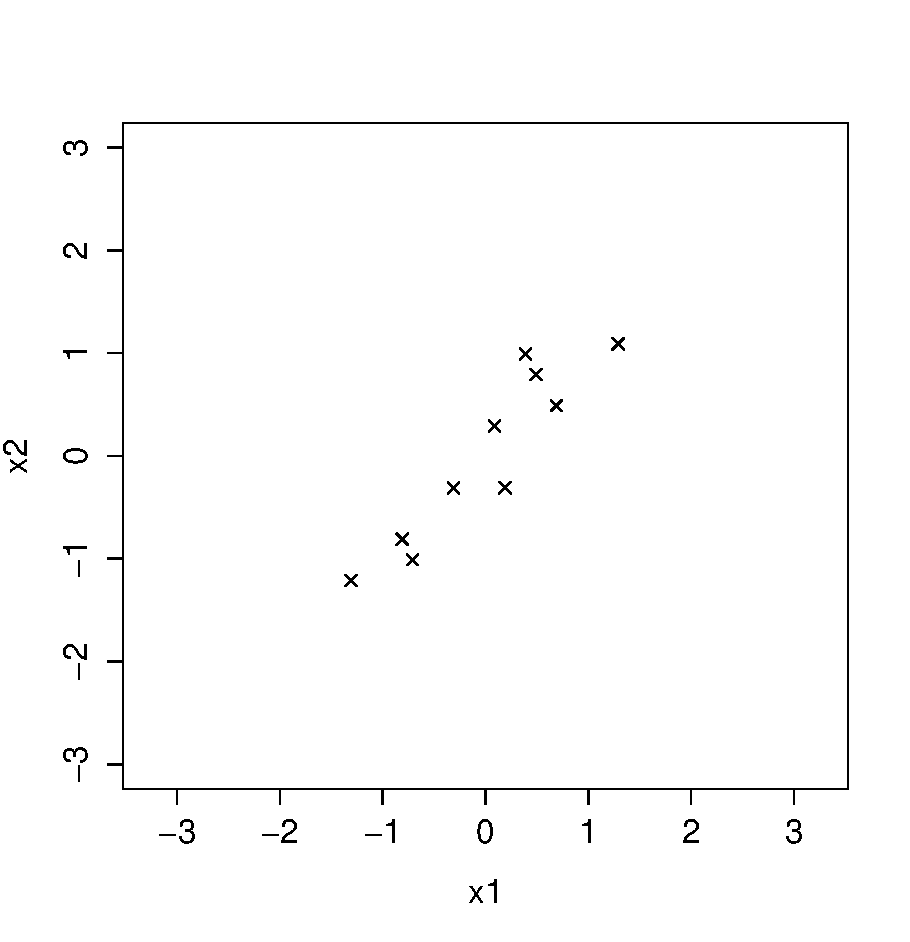
\includegraphics[width=\columnwidth]{images/points_scaled}
  \caption{Punti con media azzerata}
  \label{fig:punti_scalati}
\end{subfigure}
\caption{Campioni a cui applicare la PCA }
\label{fig:PCA}
\end{figure}



\begin{esempio}
Chiariamo la procedura tramite un esempio numerico\footnote{Esempio trattato a lezione e preso da \href{http://www.cs.otago.ac.nz/cosc453/student_tutorials/principal_components.pdf}{qui}.} eseguito in R. I dati a disposizione sono rappresentati dalle seguenti coppie di punti (\autoref{fig:punti_iniziali}):
\begin{lstlisting}
> show (dataset)
    x1  x2
1  2.5 2.4
2  0.5 0.7
3  2.2 2.9
4  1.9 2.2
5  3.1 3.0
6  2.3 2.7
7  2.0 1.6
8  1.0 1.1
9  1.5 1.6
10 1.1 0.9
\end{lstlisting} 
Eseguiamo ora i passi della PCA:
\begin{enumerate}
\item \emph{Azzeramento della media}, che effettuiamo tramite la funzione \texttt{scale}, per ottenere la nuova matrice degli ingressi con le medie azzerate (mostrati in \autoref{fig:punti_scalati}):
\begin{lstlisting}
> scaled.dataset <- scale(dataset, TRUE, FALSE)
> show(scaled.dataset)
         x1    x2
 [1,]  0.69  0.49
 [2,] -1.31 -1.21
 [3,]  0.39  0.99
 [4,]  0.09  0.29
 [5,]  1.29  1.09
 [6,]  0.49  0.79
 [7,]  0.19 -0.31
 [8,] -0.81 -0.81
 [9,] -0.31 -0.31
[10,] -0.71 -1.01
\end{lstlisting}

\item \emph{Calcolo della matrice delle covarianze}:
\begin{lstlisting}
>  Sigma <- cov(scaled.dataset)
>  show(Sigma)
          x1        x2
x1 0.6165556 0.6154444
x2 0.6154444 0.7165556
\end{lstlisting}

\item \emph{Decomposizione ai valori singolari}:
 \begin{lstlisting}
> results <- svd(Sigma)
>  show(results)
$d
[1] 1.2840277 0.0490834

$u
           [,1]       [,2]
[1,] -0.6778734 -0.7351787
[2,] -0.7351787  0.6778734

$v
           [,1]       [,2]
[1,] -0.6778734 -0.7351787
[2,] -0.7351787  0.6778734
\end{lstlisting}

Notiamo che l'\emph{output} è costuito da un vettore e due matrici. Il vettore (\texttt{d}) contiene i due autovalori (è la diagonale principale di $S$), mentre le matrici (\texttt{u} e \texttt{v}) contengo rispettivamente gli autovettori sinistri e destri, uno per colonna, e corrispondono quindi ad $U$ e $V$ (non $V^*$). Notiamo anche che, essendo $\Sigma$ reale, accade che $u = v$.

\item \emph{Proiezione dei dati sul nuovo sistema di riferimento}. Volendo ridurre il numero di \emph{feature} da $2$ ad $1$, ci limitiamo a considerare l'autovalore più grande (il primo) ed il corrispondente autovettore (la prima colonna di \texttt{u} o \texttt{v}).
A questo punto moltiplichiamo la matrice dei campioni per questo autovettore ed otteniamo le coordinate dei punti nel nuovo spazio:
\begin{lstlisting}
> new.dataset <- scaled.dataset %*% results$u[,1] 
> show(new.dataset)
             [,1]
 [1,] -0.82797019
 [2,]  1.77758033
 [3,] -0.99219749
 [4,] -0.27421042
 [5,] -1.67580142
 [6,] -0.91294910
 [7,]  0.09910944
 [8,]  1.14457216
 [9,]  0.43804614
[10,]  1.22382056
\end{lstlisting}



\end{enumerate}

A questo punto la PCA è conclusa ma, poiché stiamo lavorando con punti del piano, possiamo visualizzare graficamente quali siano le due componenti individuate. Per disegnare ciascuna componente è sufficiente sovrappore al \emph{plot} dei punti (scalati) la retta con intercetta nulla e coefficiente angolare pari al rapporto tra il primo ed il secondo elemento dell'autovettore (equivalentemente si potrebbero usare i punti iniziali e \emph{plottare} questa retta con le coordinate traslate di una quantità pari alle medie sottratte in partenza).
\begin{lstlisting}
plot(scaled.dataset, pch = 4, xlim = c(-3,3), ylim = c(-3,3))

m1 <-  results$u[,1][1] / results$u[,1][2] 
comp1 <- matrix(c(seq(-3,3), m1*seq(-3,3)), 7, 2)
points(comp1, col="red", type = "l")

m2 <-  results$u[,2][1] / results$u[,2][2] 
comp2 <- matrix(c(seq(-3,3), m2*seq(-3,3)), 7, 2)
points(comp2, col="blue", type = "l" )
\end{lstlisting}
Il risultato è mostrato in \autoref{fig:components_scaled}. Effettivamente notiamo che le proiezioni dei punti sulla prima componente (disegnata in rosso) hanno varianza maggiore. Verifichiamo se quest'ultima affermazione è vera calcolando le varianze delle proiezioni dei punti sui due assi:
\begin{lstlisting}
> var(scaled.dataset %*% results$u[,1])
         [,1]
[1,] 1.284028
> var(scaled.dataset %*% results$u[,2])
          [,1]
[1,] 0.0490834
\end{lstlisting}
Questi risultati confermano quanto ci aspettavamo e notiamo che la varianza lungo ciascuna componente è pari proprio all'autovalore che determina tale componente (motivo per cui prendiamo in considerazione gli autovalori più grandi).

\begin{figure}[tbp]
\centering
  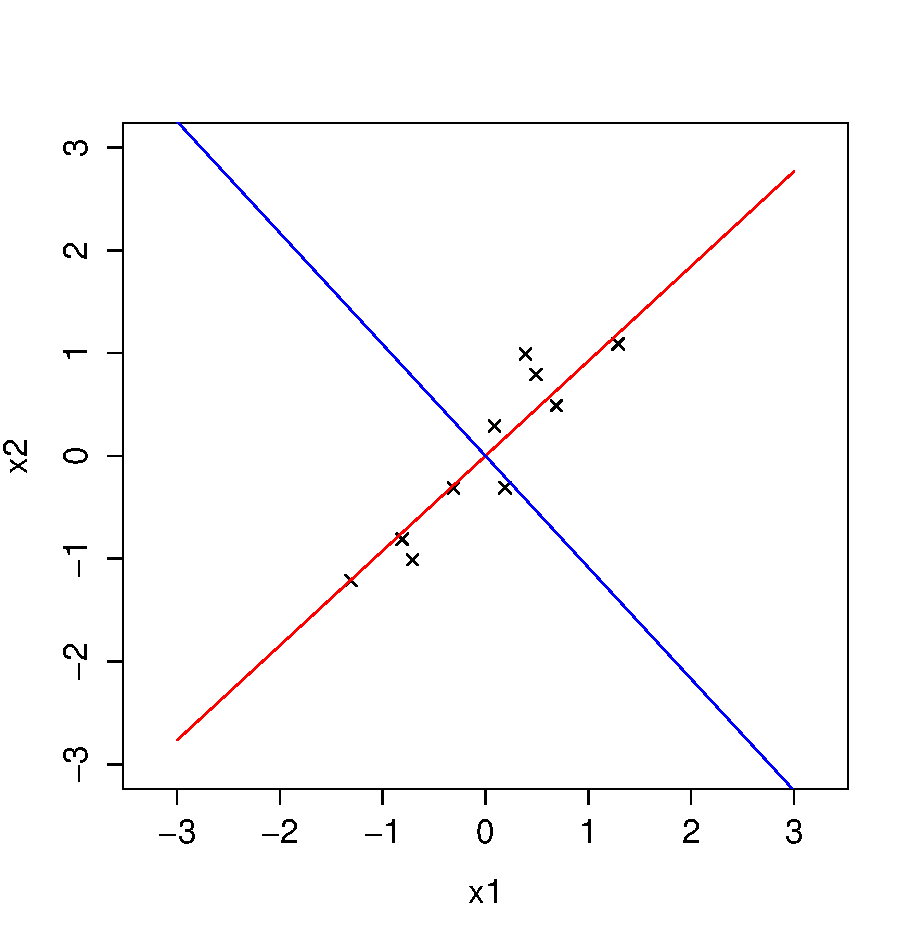
\includegraphics[width=0.5\textwidth]{images/components_scaled}
  \caption{Componenti individuate tramite PCA}
  \label{fig:components_scaled}
\end{figure}
\end{esempio}

\subsubsection{Scelta del numero di componenti principali}\label{scelta-p}
Fin qui non abbiamo detto niente su quante componenti prendere in considerazione, cioè su come determinare il parametro $p$. Una regola comunemente usata\footnote{{\href{https://class.coursera.org/ml-005/lecture/86}{Coursera, Machine Learning (Andrew Ng), Lezione 8.5}}} è individuare il più piccolo $p$ che garantisce la seguente disuguaglianza:
\begin{equation*}
\displaystyle\frac{\displaystyle\frac{1}{m} \sum_{i=1}^m || x^{(i)} - \hat{x}^{(i)}||^2}{\displaystyle\frac{1}{m} \sum_{i=1}^m || x^{(i)}||^2} \leq 1-\epsilon
\end{equation*}
dove $\hat{x}^{(i)}$ rappresenta la proiezione del punto $x^{(i)}$ sull'iperpiano individuato dalle prime $p$ componenti (nota che le coordinate di $\hat{x}^{(i)}$ sono ancora espresse rispetto al sistema di riferimento originale, altrimenti questa distanza non avrebbe senso). Il numeratore della precedente equazione rappresenta quindi la distanza quadratica media tra ciascun punto e la sua proiezione sull'iperpiano in $p$ dimensioni, mentre il denominatore rappresenta la lunghezza media dei vettori che uniscono l'origine a ciascun punto. Valori tipici per $\epsilon$ sono compresi tra $0.95$ e $0.99$, ma si può arrivare anche a $0.85$ in casi particolari. Se ad esempio troviamo un valore di $p$ per $\epsilon = 0.99$ possiamo affermare che dopo la PCA abbiamo \emph{mantenuto il 99\% della varianza}.
Il valore di $p$ può essere quindi determinato iterativamente, partendo da $p=1$ ed eventualmente incrementandolo fintanto che la diseguaglianza vista in precedenza non risulti vera. Questa formulazione del problema, però, richiede il calcolo delle proiezioni di tutti gli $m$ campioni per ogni valore di $p$ che stiamo testando. Matematicamente si dimostra che:
\begin{equation*}
\displaystyle\frac{\displaystyle\frac{1}{m} \sum_{i=1}^m || x^{(i)} - \hat{x}^{(i)}||^2}{\displaystyle\frac{1}{m} \sum_{i=1}^m || x^{(i)}||^2} = 1 - \displaystyle\frac{\displaystyle\sum_{i=1}^p \lambda_i}{\displaystyle\sum_{i=1}^n \lambda_i}
\end{equation*}
dove $\lambda_i$ rappresenta l'\emph{i-esimo} autovalore della matrice delle covarianze. La disuguaglianza precedente diventa quindi:
\begin{equation*}
\displaystyle\frac{\displaystyle\sum_{i=1}^p \lambda_i}{\displaystyle\sum_{i=1}^n \lambda_i} \geq \epsilon
\end{equation*}
Questo risultato ci consente di determinare $p$ senza calcolare le proiezioni dei punti, infatti gli autovalori sono tutti presenti sulla diagonale principale della matrice $S$ ed il numeratore della precedente è la somma dei primi $p$ autovalori, mentre il denominatore è la somma dell'intera diagonale.

In definitiva la procedura di selezione di $p$ può essere sintetizzata come segue:
\begin{enumerate}
\item Ottieni la matrice $S$ tramite SVD ed inizializza $p = 1$;
\item La seguente disuguaglianza è vera?
\begin{equation*}\frac{\sum_{i=1}^p \lambda_i}{\sum_{i=1}^n \lambda_i} \geq \epsilon\end{equation*}
\begin{itemize}
\item Se sì, abbiamo trovato il valore desiderato di $p$;
\item Altrimenti incrementa $p$ e torna al passo 2;
\end{itemize}
\end{enumerate}

\clearpage
\subsection{Soft clustering tramite GMM}

In questo capitolo esamineremo i \emph{mixture model}. Si tratta di modelli probabilistici, cioè di funzioni densità di probabilità, ottenuti dalla somma pesata di densità di probabilità elementari. In particolare ci occuperemo di \emph{Gaussian Mixture Model} (GMM) cioè di modelli probabilistici ottenuti dalla somma pesata di un certo numero di funzioni gaussiane. L'ambito in cui applicheremo le GMM è il \emph{soft clustering}, cioè esamineremo una procedura, basata sull'utilizzo di GMM, che sia in grado di dirci qual è la probabilità che un punto appartenga a ciascun \emph{cluster} individuato in una nuvola di punti.


\begin{figure}[h]
\centering
\begin{subfigure}[b]{0.5\textwidth}
    \centering
    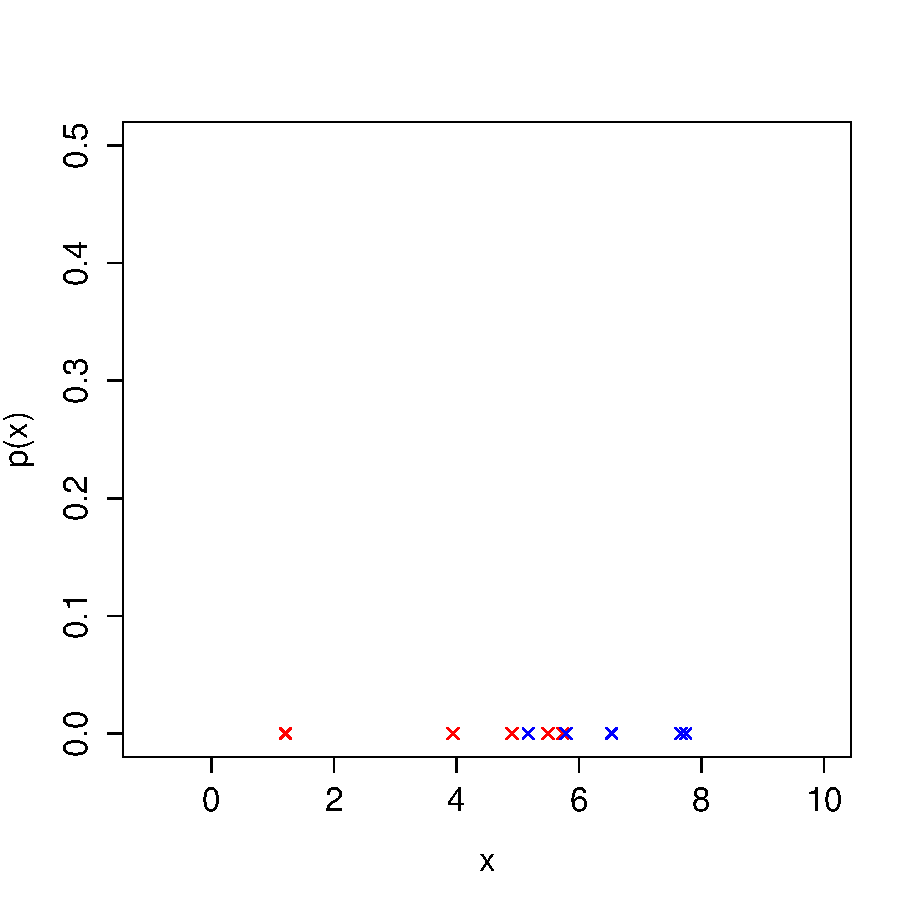
\includegraphics[width=\columnwidth]{images/gmm_points}
    \caption{}
    \label{fig:gmm_points}
\end{subfigure}%
\begin{subfigure}[b]{0.5\textwidth}
    \centering
    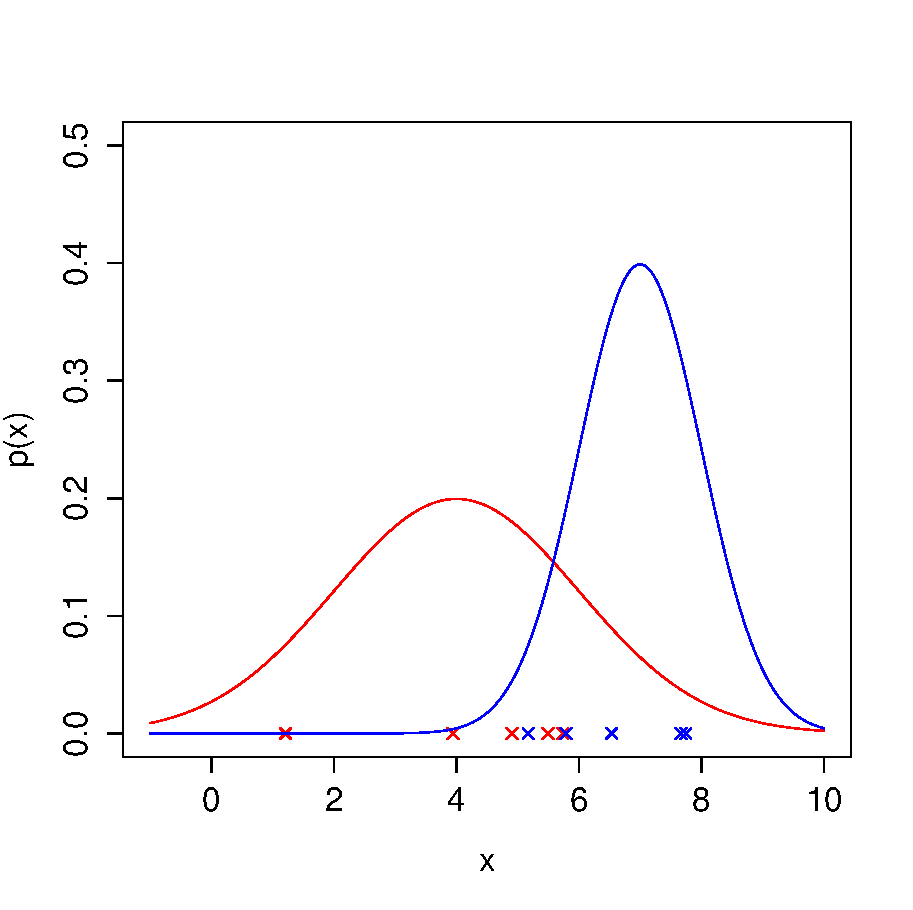
\includegraphics[width=\columnwidth]{images/gmm_gaussians}
    \caption{}
    \label{fig:gmm_gaussians}
\end{subfigure}
\caption{Punti da \emph{clusterizzare} e gaussiane da cui sono stati estratti.}
\label{fig:gmm_example}
\end{figure}


\subsubsection{L'idea in sintesi}
Per capire l'approccio adottato partiamo da un semplice esempio. Ipotizziamo di voler effettuare il \emph{clustering} di un certo numero di punti caratterizzati da una sola coordinata. Essi sono rappresentabili su una retta, come mostrato sull'asse $x$ in \autoref{fig:gmm_points}. Per comodità i punti di ciascun \emph{cluster} sono rappresentati con un colore differente. Ipotizziamo che i punti appartenenti a ciascun \emph{cluster} siano distribuiti come se fossero stati estratti da una gaussiana. Quindi, nel nostro esempio, avremo due gaussiane con parametri diversi tra di loro (\autoref{fig:gmm_gaussians}). Se riuscissimo a determinare tali parametri, saremmo in grado di calcolare la probabilità che un nuovo punto sia stato generato dalla prima o dalla seconda gaussiana. Ciò significherebbe conoscere la probabilità che il punto appartenga al primo \emph{cluster} e la probabilità che appartenga al secondo \emph{cluster}, ovvero avremmo realizzato \emph{soft clustering}.

Per determinare i parametri delle due gaussiane operiamo direttamente sul GMM corrispondente, cioè stiamo ipotizzando che i punti da \emph{clusterizzare} siano stati generati da un GMM. In prima analisi potremmo immaginarlo come la somma delle due gaussiane, così come mostrato dalla linea tratteggiata in \autoref{fig:gmm_gmm}. Tuttavia sorge un problema: come ben noto l'area sottesa da ciascuna gaussiana è unitaria, quindi l'area sottesa dalla loro somma non lo sarà. Affinché il GMM sia un modello probabilistico, ovvero affinché sia una densità di probabilità, è necessario che sottenda anch'esso un'area unitaria. Per tale motivo ciascuna delle gaussiane di partenza viene moltiplicata per una quantità compresa tra $0$ ed $1$ prima di essere sommata alle altre. Intuitivamente questo giustifica il fatto che un GMM sia una somma pesata di distribuzioni elementari. Vedremo in seguito che significato fisico è possibile dare a questi pesi.

\begin{figure}[tbp]
\centering
  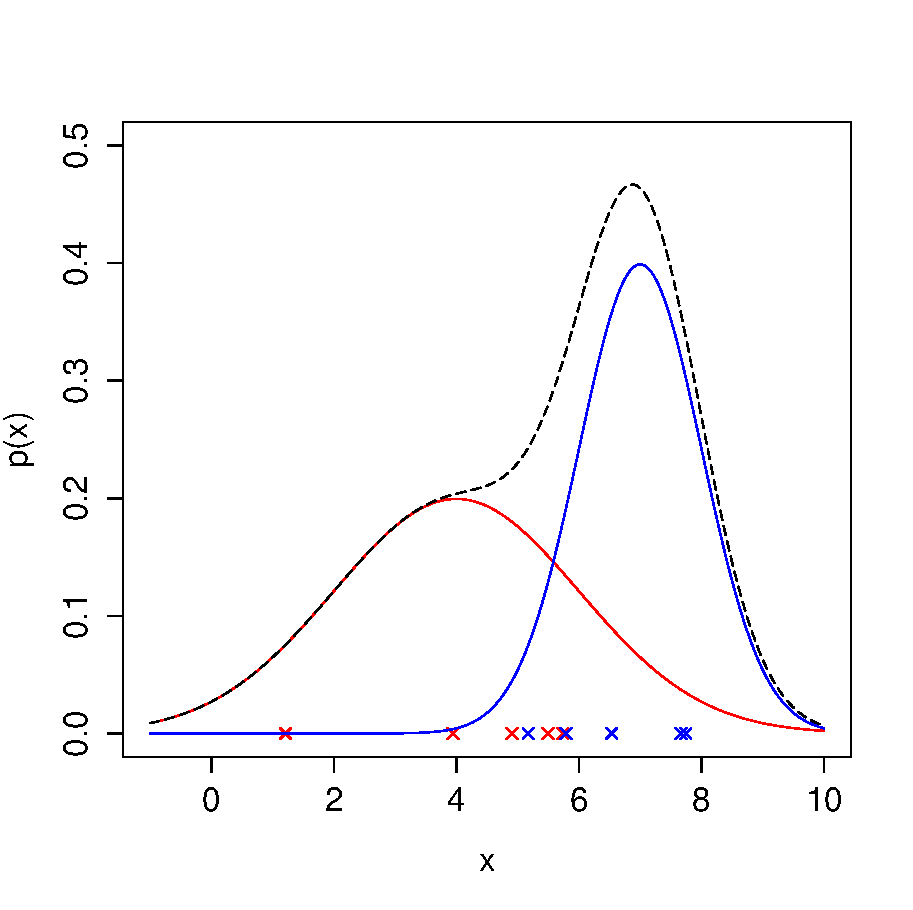
\includegraphics[width = 0.5\columnwidth]{images/gmm_gmm}
  \caption{Somma delle due gaussiane.}
  \label{fig:gmm_gmm}
\end{figure}


Il caso esaminato fin qui prevede che ciascun punto sia descritto da una sola coordinata. Nel caso di punti a $2$ o più variabili l'idea di fondo rimane invariata, mentre cambiano alcuni dettagli. In particolare non potremo più usare una semplice distribuzione gaussiana univariata, ma dovremo ricorrere ad una gaussiana multivariata. Nel caso in cui i punti da \emph{clusterizzare} si trovino sul piano ($n=2$) la mistura di gaussiane assume una forma simile a quella mostrata in \autoref{fig:esempio_GMM}. In essa è rappresentato un GMM formato da $3$ distribuzioni gaussiane bidimensionali (o bivariate).



\begin{figure}[tbp]
\centering
  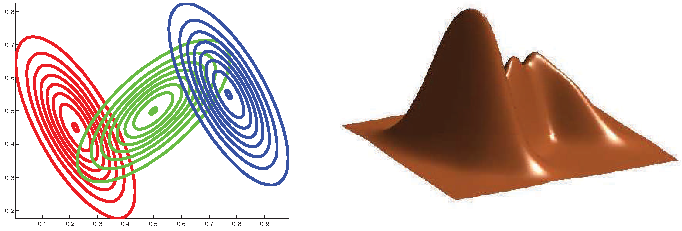
\includegraphics[width = 0.8\textwidth]{images/esempio_GMM}
  \caption{Esempio di GMM con 3 gaussiane bivariate}
  \label{fig:esempio_GMM}
\end{figure}

\subsubsection{Dettagli matematici}
Nei paragrafi che seguono formalizziamo meglio il problema ed approfondiamo alcuni dettagli. 

\paragraph{Mixture model in formule}
Fin qui abbiamo definito una mistura di gaussiane come una somma pesata di densità di probabilità gaussiane. Più in generale possiamo parlare di \emph{Mixture Model} come una somma pesata di densità di probabilità, senza specificarne la natura. Ipotizzando di voler creare una mistura con $k$ componenti, la formulazione più generica per la densità di probabilità del modello è\footnote{Per una formulazione più formale vedi \href{http://www.youtube.com/watch?v=Rkl30Fr2S38}{qui}.}:

\begin{equation*}
p(\mathbf{x}) = \sum_{j=1}^k p(\mathbf{x} \land z = j).
\end{equation*}
Nella precedente $p(\mathbf{x} \land z = j)$ rappresenta la probabilità che il punto $\mathbf{x}$ sia stato generato dalla \emph{j-esima} componente. Applicando la regola del prodotto possiamo riscriverla nella formulazione tipicamente usata:
\begin{equation*}
p(\mathbf{x}) = \sum_{j=1}^k p(\mathbf{x}| z = j) p(z = j).
\end{equation*}
In essa $z$ rappresenta una variabile casuale discreta (latente) che assume valori da $1$ a $k$. $p(z=j)$ indica la probabilità che la \emph{j-esima} componente della mistura venga ``attivata'' e generi il campione.
A livello intuitivo possiamo pensare al processo di generazione di un punto in questa maniera:
\begin{itemize}
\item la componente \emph{j-esima} viene selezionata per la generazione del punto con una probabilità $p(z=j)$;
\item il punto viene generato dalla componente \emph{j-esima} con una probabilità $p(\mathbf{x}|z=j)$ che dipende \emph{solo} dalla natura di questa componente (cioè dalla sua specifica distribuzione di probabilità).
\end{itemize}
In definitiva, possiamo vedere la precedente formula come una risposta alla domanda:
\begin{itemize}
\item ``Con quale probabilità la mistura può generare un punto $\mathbf{x}$?''
\end{itemize}
La risposta fornita dalla formula è:
\begin{itemize}
\item ``Per ciascuna distribuzione, considera la probabilità che sia essa a generare quel punto e moltiplicala per la probabilità con cui essa lo genererebbe. In seguito somma tutte queste quantità e saprai con che probabilità la mistura darà vita al punto $\mathbf{x}$.''
\end{itemize}

A questo punto possiamo semplificare la notazione introducendo i coefficienti $\pi_j = p(z=j)$ che ci consentono di scrivere: 
\begin{equation*}
p(\mathbf{x}) = \sum_{j=1}^k \pi_j p_j(\mathbf{x}).
\end{equation*}
$p_j(\mathbf{x}$) rappresenta la densità di probabilità della \emph{j-esima} componente calcolata nel punto $\mathbf{x}$, mentre i vari $\pi_j$ prendono il nome di \emph{mixing coefficients} e sono proprio i pesi di cui abbiamo parlato finora. Notiamo anche che, trattandosi di valori di probabilità, la loro somma è unitaria:
\begin{equation*}
\sum_{j=1}^k\pi_j= \sum_{j=1}^k p(z=j) = 1.
\end{equation*}

Poiché il nostro scopo sarà individuare i parametri migliori per le singole distribuzioni, conviene adottare una notazione più esplicita, cioè la seguente:

\begin{equation*}
p(\mathbf{x}|\boldsymbol{\theta}) = \sum_{j=1}^k \pi_j p_j(\mathbf{x} | \boldsymbol{\theta_j})
\end{equation*}
in cui $\boldsymbol\theta_j$ rappresenta i parametri della componente \emph{j-esima}, ad esempio media e varianza di una gaussiana univariata, mentre $\boldsymbol\theta$ è una particolare istanza di tutti i parametri $\boldsymbol\theta_j$.

\paragraph{Parametri di un GMM}
Fin qui abbiamo parlato genericamente di ``parametri'' di un modello. Scendiamo ora nel dettaglio delle GMM. Il primo passo da fare è sostituire la generica densità di probabilità $p_j(\mathbf{x} | \boldsymbol{\theta_j})$ con la \emph{j-esima} gaussiana multivariata, la cui espressione è:

\begin{equation*}
\mathcal{N}(\mathbf{x} | \boldsymbol{\mu_j}, \boldsymbol{\Sigma_j}) = \frac{1}{\sqrt{(2\pi)^{n} |\boldsymbol\Sigma_j|}} \exp\left(-\frac{1}{2}({\mathbf x}-{\boldsymbol\mu_j})^T{\boldsymbol\Sigma_j}^{-1}({\mathbf x}-{\boldsymbol\mu_j})
\right)
\end{equation*}
nella quale:
\begin{itemize}
\item $n$ rappresenta la dimensione di ciascun ingresso (e quindi il numero di \emph{feature});
\item $\boldsymbol\mu_j$ è il vettore dei valori medi della \emph{j-esima} gaussiana;
\item $\boldsymbol\Sigma_j$ è la matrice delle covarianze della \emph{j-esima} gaussiana.
\end{itemize}
I parametri che desideriamo individuare sono quindi:
\begin{gather*}
\boldsymbol\mu_j \text{~e~} \boldsymbol\Sigma_j \quad j=1, \dots, k.
\end{gather*}

Nel caso di gaussiane univariate questi si riducono ai valori medi ($\mu_j$) ed alle varianze ($\sigma^2_j$). Se per ogni \emph{cluster} sapessimo quali punti appartengono ad esso, potremmo calcolare le stime di media e varianza tramite le formule note:
\begin{gather*}
\hat\mu_j = \frac{1}{|C_j|} \sum_{ x^{(i)} \in C_j} x^{(i)} \\
\hat\sigma^2_j = \frac{1}{|C_j|-1} \sum_{x^{(i)} \in C_j}(x^{(i)}- \hat\mu_j)^2
\end{gather*}
dove ${C_j}$ rappresenta il \emph{j-esimo} \emph{cluster} e $|{C_j}|$ è il numero di punti di cui è composto. Chiaramente lo stesso discorso può essere esteso al caso multivariato:
\begin{gather*}
\boldsymbol{\hat\mu_j} = \frac{1}{|C_j|} \sum_{ \mathbf{x^{(i)}} \in C_j} \mathbf{x^{(i)}} \\
\hat\Sigma_j = \frac{1}{|C_j|-1} \sum_{\mathbf{x^{(i)}} \in C_j}(\mathbf{x^{(i)}}- \boldsymbol{\hat\mu_j})(\mathbf{x^{(i)}}- \boldsymbol{\hat\mu_j})^T
\end{gather*}
Purtroppo, però, non è noto a priori quali punti siano stati generati da ciascun cluster, altrimenti il problema del \emph{clustering} non si porrebbe neppure. Potremmo quindi pensare di assegnare ciascun punto ad un \emph{cluster} in base alla gaussiana a cui appartiene con maggiore probabilità. Fare ciò, tuttavia, richiederebbe di conoscere i parametri delle gaussiane, che non sono affatto noti. Ci troviamo quindi in questa situazione:
\begin{itemize}
\item per stimare i parametri di ciascuna gaussiana dovremmo conoscere i punti che le appartengono;
\item per conoscere i punti che appartengono a ciascuna gaussiana dovremmo stimarne i parametri.
\end{itemize}
La procedura che risolve questo problema si chiama \emph{Expectation-Maximization} (EM).

\paragraph{Algoritmo EM per GMM}

L'algoritmo EM applicato ad un GMM può essere sintetizzato nei seguenti passaggi\footnote{I dettagli sulle formule sono in ``Machine Learning - A Probabilistic Perspective'', Sezione 11.4.2}:
\begin{enumerate}
    \item fissato $k$ inizializza casualmente i parametri delle gaussiane ed i pesi $\pi_j$;
    \item passo E (\emph{Expectation}): per ogni coppia punto-\emph{cluster} calcola alcuni coefficienti, detti \emph{responsibility}, definiti come segue:
        \begin{equation*}
r_{ij}\triangleq p(z=j | \mathbf{x^{(i)}}, \boldsymbol\theta^{t-1})
        \end{equation*}
 dove $\boldsymbol\theta^{t-1}$ rappresenta i parametri del modello all'iterazione precedente. Ciascun coefficiente tiene conto di quanto il \emph{cluster} \emph{j-esimo} sia responsabile del punto \emph{i-esimo} ed è calcolato come il rapporto tra la probabilità che il punto sia stato generato dal \emph{cluster} e quella che sia stato generato dall'intero GMM:
         \begin{equation*}
r_{ij} =\frac{\pi_j p_j(\mathbf{x}^{(i)} | \boldsymbol{\theta_j}^{(t-1)})}{ \sum_{j=1}^k \pi_j p_j(\mathbf{x}^{(i)}  | \boldsymbol{\theta_j}^{(t-1)})}
         \end{equation*}
    \item passo M (\emph{Maximization}): per ogni gaussiana ricalcola i parametri $\pi_j$, $\boldsymbol\mu_j$ e $\boldsymbol\Sigma_j$ in base alle \emph{responsibility} appena calcolate, con lo scopo di massimizzare la \emph{likelihood} (cioè la probabilità che quei punti siano stati generati dal GMM):
        \begin{gather*}
            \pi_j = \frac{1}{m} \sum_{i=1}^m r_{ij} \\
           \boldsymbol{\mu_j} = \frac{\sum_{i} r_{ij}\mathbf{x^{(i)}}}{\sum_{i} r_{ij}} \\
            \mathbf{\Sigma_j} = \frac{\sum_{i} r_{ij} (\mathbf{x}^{(i)} - \boldsymbol{\mu_j})(\mathbf{x}^{(i)} - \boldsymbol{\mu_j})^T} {\sum_{i} r_{ij}}
    \end{gather*}
\item ripeti i passi E ed M fino a convergenza.
\end{enumerate}

%Come già accennato, l'idea dei modelli basati su variabili latenti è che l'insieme di variabili osservabili sia deducibile a partire da un insieme più piccolo di variabili latenti\footnote{Machine Learning - A Probabilistic Perspective, Capitolo 11}. Se chiamiamo $z_i$ le variabili latenti ed $x_i$ quelle osservabili possiamo distinguere i seguenti modelli:
%\begin{itemize}
%\item \emph{molti a molti}, in cui ciascuna variabile latente influisce su più variabili osservabili e ciascuna variabile osservabile subisce l'influenza di più variabili latenti;
%\item \emph{uno a molti}, in cui una variabile latente influisce su più variabili osservabili;
%\item \emph{molti ad uno}, in cui più variabili latenti influiscono su una singola variabile osservabile;
%\item \emph{uno ad uno}, in cui una variabile latente influisce su una sola variabile osservabile.
%
%\end{itemize}
%\begin{figure}[tbp]
%\centering
%  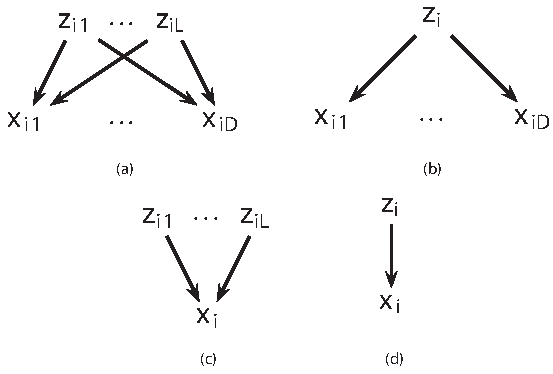
\includegraphics[width = 0.6\textwidth]{images/cardinalita_modelli_latenti}
%  \caption{Possibili cardinalità della relazione $z_i \rightarrow x_i$}
%\label{fig:cardinalita_modelli_latenti}
%\end{figure}
%
%Assumendo che $\mathbf{x_i}$ e $\mathbf{z_i}$ possano essere vettori, la notazione $\mathbf{z_i} \rightarrow\mathbf{x_i}$ riassume tutti i casi precedenti. A questo punto possiamo definire:
%\begin{itemize}
%\item $p(\mathbf{x_i}| \mathbf{z_i})$ come la probabilità che un'istanza di variabili osservabili $\mathbf{x_i}$ venga generata a partire da un'istanza di variabili latenti $\mathbf{z_i}$ (detta \emph{likelihood});
%\item $p(\mathbf{z_i})$ probabilità a priori delle variabili latenti.
%\end{itemize}
%A seconda della scelta delle due distribuzioni si possono generare diversi modelli.

%\subsection{Forma generale}
%Una forma generale e semplice per descrivere un \emph{mixture model} è questa\footnote{Vedi anche AIMA, Capitolo 20.3.}:
%\begin{equation*}
%p(\mathbf{x_i}|\theta) = \sum_{k=1}^K \pi_k p_k(\mathbf{x_i}|\theta)
%\end{equation*}
%in cui:
%\begin{itemize}
%\item $p(\mathbf{x_i}|\theta)$ rappresenta la probabilità che i dati a disposizione $\mathbf{x_i}$ vengano generati da un modello probabilistico i cui parametri sono $\theta$;
%\item $K$ rappresenta il numero di possibili stati latenti (discreti), che nel caso del \emph{clustering} corrisponderà al numero di \emph{cluster};
%\item $\pi_k$ sono dei coefficienti numerici che fungono da pesi, tali che $0\leq\pi_k\leq1$ e $\sum_k(\pi_k)=1$, se pensiamo all'estrazione di un punto dal modello possiamo vederli come la probabilità che un campione venga generato a partire dalla \emph{k-esima} componente della mistura;
%\item $ p_k(\mathbf{x_i}|\theta)$ rappresenta la distribuzione di probabilità del \emph{k-esimo} stato latente, fissati i parametri $\theta$.
%\end{itemize}
%
%Applicando questo modello al \emph{clustering} (\emph{soft clustering} per l'esattezza) stiamo facendo ciò: ipotizziamo che siano presenti $K$ \emph{cluster},  ciascuno di essi è rappresentato da una densità di probabilità. Per ciascun campione calcoliamo la probabilità che esso appartenga a ciascun cluster, cioè a ciascuna distribuzione di probabilità (\emph{responsibility}), e qui terminerebbe il \emph{clustering}. Per capire il significato dell'espressione precedente, consideriamo che, intuitivamente, sommando le probabilità appena descritte otterremmo la probabilità che quel campione sia stato assegnato con un certo grado di certezza ad almeno un \emph{cluster}. Tuttavia la somma sarebbe maggiore di 1, e non potrebbe rappresentare una probabilità essa stessa, quindi facciamo una somma pesata secondo i coefficienti $\pi_k$. 
%
%Quindi, se accade che $p(\mathbf{x_i}|\theta)$ è piccolo, signfica che non c'è alcun \emph{cluster}  al quale si può ``scommettere'' che l'istanza appartenga, perché mediamente esso appartiene a ciascun \emph{cluster} con una probabilità molto bassa. L'ideale si ha quando la somma di queste probabilità su tutte le istanze è alta, cioè quando bene o male per ciascun campione ho individuato uno o più \emph{cluster} a cui esso appartiene ``abbastanza probabilmente''.
%
%\subsection{Gaussian Mixture Model}
%Nel caso di GMM la probabilità che un punto appartenga a ciascun \emph{cluster} è gaussiana multivariata (cioè in più dimensioni), dall'espressione:
%\begin{equation*}
%\mathcal{N}(\mathbf{x}_i|\boldsymbol{\mu}_k, \boldsymbol\Sigma_k) = \frac{1}{\sqrt{(2\pi)^{D} |\boldsymbol\Sigma_k|}} \exp\left(-\frac{1}{2}({\mathbf x_i}-{\boldsymbol\mu_k})^T{\boldsymbol\Sigma_k}^{-1}({\mathbf x_i}-{\boldsymbol\mu_k})
%\right)
%\end{equation*}
%in cui:
%\begin{itemize}
%\item $D$ rappresenta la dimensione di ciascun ingresso (e quindi il numero di dimensioni della gaussiana);
%\item $\boldsymbol\mu_k$ il vettore dei valor medi della \emph{k-esima} gaussiana;
%\item $\boldsymbol\Sigma_k$ la matrice delle covarianze della \emph{k-esima} gaussiana.
%\end{itemize}
%Il modello GMM è quindi:
%\begin{equation*}
%p(\mathbf{x_i}|\theta) = \sum_{k=1}^K \pi_k \mathcal{N}(\mathbf{x}_i|\boldsymbol{\mu}_k, \boldsymbol\Sigma_k).
%\end{equation*}
%In~\autoref{fig:esempio_GMM} è mostrato un esempio grafico di come può apparire il modello con $k=3$ e $D=2$.
%
%
%
%Il problema in tutto ciò è come determinare i parametri $\boldsymbol\mu_k$ e $\mathbf\Sigma_k$ per ciascuna gaussiana quando facciamo \emph{clustering}. Infatti a priori non abbiamo informazioni a sufficienza, ovvero:
%\begin{itemize}
%\item per determinare la probabilità con cui ciascun punto appartiene a ciascuna gaussiana dovremmo conoscere i parametri delle gaussiane;
%\item per determinare i parametri delle gaussiane dovremmo sapere quali punti appartengono a ciascuna di esse.
%\end{itemize}
%


\subsection{Outlier detection tramite densità di probabilità}
La gaussiana multivariata può essere usata anche per fare \emph{outlier detection}. Partendo da un \emph{dataset} noto, ed ipotizzando che i campioni siano stati estratti da una distribuzione gaussiana, è possibile calcolare le stime dei parametri, come mostrato in precedenza. Prendendo come caso d'esempio quello della gaussiana univariata, sappiamo che sommando e sottraendo alla media 3 deviazioni standard ($\mu \pm 3 \sigma$) otteniamo i due estremi dell'intervallo in cui ricade il 99.7\% dei campioni (\autoref{fig:outlier_detection}). Data questa informazione possiamo classificare come \emph{outlier} tutte le istanze del \emph{dataset} che fuoriescono dall'intervallo stabilito. Ovviamente il discorso può essere ripetuto per gaussiane multivariate.
\begin{figure}[h]
\centering
  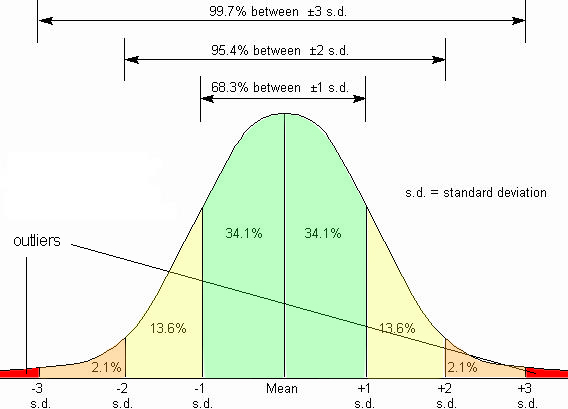
\includegraphics[width=0.65 \textwidth]{images/outlier_detection}
  \caption{\emph{Outlier detection} tramite gaussiana univariata}
  \label{fig:outlier_detection}
\end{figure}


